% HAFF: Holographic Alaya-Field Framework
% Paper A: Emergent Geometry from Coarse-Grained Observable Algebras
% CORRECTED VERSION (Post-Review)

\documentclass[12pt,a4paper]{article}
\usepackage{arxiv}
\usepackage{amsmath,amssymb,amsfonts,amsthm}
\usepackage{physics}
\usepackage{graphicx}
\usepackage{hyperref}
\usepackage{tikz}
\usetikzlibrary{shapes,arrows}
\usepackage{bbm}

% Theorem environments
\newtheorem{theorem}{Theorem}[section]
\newtheorem{definition}[theorem]{Definition}
\newtheorem{remark}[theorem]{Remark}

\title{Emergent Geometry from Coarse-Grained Observable Algebras:\\
The Holographic Alaya--Field Framework}

\author{
  [Sidong Liu, PhD] \\[0.6ex]
  [iBioStratix Ltd] \\[0.8ex]
  \texttt{[sidongliu@hotmail.com]}
}

\date{\today}

\begin{document}

\maketitle

\noindent\textbf{Preliminary Remark (Structural Stance).}
In much of modern theoretical physics, it is tacitly assumed that the decomposition of a system into subsystems is either physically given or at least unproblematic. 
Hilbert spaces are factorized, degrees of freedom are labeled, and geometry is inferred from relations between these parts.

In this work, we adopt a different structural stance. 
We treat the universal quantum state as given, but regard subsystem structure, locality, and geometry as secondary constructs arising from restrictions on observable algebras. 
The guiding question is not how geometry emerges from quantum states, but how different effective realities can emerge from the \emph{same} state once no preferred factorization is assumed.

This shift is modest in formalism but radical in implication: it relocates the origin of structure from states to algebras, and from kinematics to accessibility.

\medskip

\begin{abstract}
We construct a theoretical framework where the tensor factorization of a Hilbert space is treated as a dynamical variable rather than a kinematic background. 
By lifting the ``Alaya'' concept to a globally entangled vacuum state $|\Psi_{\text{vac}}\rangle$, we demonstrate that local geometry emerges from specific observable subalgebras $\mathcal{A}_i \subset \mathcal{B}(\mathcal{H})$. 
We prove that non-commuting coarse-graining maps induce topologically distinct emergent spacetimes from the same underlying state.
The analysis is structural in nature: we do not propose new dynamics, but examine consistency and consequences of removing subsystem factorization from fundamental assumptions. 
This approach is complementary to existing interpretational frameworks and suggests natural connections to algebraic quantum field theory, entanglement-based approaches to spacetime, and quantum information theory.
\end{abstract}

\section{Introduction}

\subsection{Motivation}

Two central problems in contemporary theoretical physics concern the emergence of classicality and the emergence of geometry. 
In quantum foundations, the measurement problem asks how effectively classical behavior arises from an underlying quantum description. 
Decoherence theory has provided a powerful account of this process by explaining the suppression of interference between certain degrees of freedom through environmental entanglement \cite{Zurek2003}. 
However, this explanation typically presupposes a fixed decomposition of the total system into subsystems, distinguishing ``system,'' ``apparatus,'' and ``environment'' from the outset.

A closely related emergence problem appears in quantum gravity. 
A growing body of work suggests that spacetime geometry is not fundamental, but arises from patterns of quantum entanglement \cite{Maldacena1999,VanRaamsdonk2010}. 
In holographic settings, geometric quantities are related to entanglement measures via precise correspondences, most notably the Ryu--Takayanagi formula \cite{RyuTakayanagi2006}. 
Yet these constructions likewise assume a prior specification of spatial regions or tensor factors, with geometry inferred only after such a subdivision has been fixed.

In both contexts, the emergence problem is addressed only after a subsystem decomposition has been assumed.
The structure responsible for classicality or geometry is therefore explained relative to a partition whose origin remains largely unexamined.

\subsection{The Structural Gap}

The assumption of a given subsystem structure is often treated as innocuous, or as a matter of convenient description. 
However, from a fundamental perspective, there is no canonical tensor factorization of a generic Hilbert space, nor a unique way to decompose a global quantum state into subsystems.
While this issue is occasionally acknowledged in passing \cite{Zanardi2004,Viola2004}, its consequences for emergence are rarely explored systematically.

The present work does not challenge the empirical success of decoherence theory, entanglement-based approaches to geometry, or the algebraic formulation of quantum theory.
Rather, we make explicit a structural assumption common to these frameworks and investigate the consequences of relaxing it.
Our focus is on what follows if subsystem structure itself is treated as emergent, rather than fundamental.

\subsection{Our Contribution}

We formulate a framework in which subsystem structure is not assumed \emph{a priori}, but arises from a choice of coarse-graining over observable algebras.
Within this framework, we show that different coarse-grainings of the same global quantum state generically induce inequivalent effective geometries.
We further clarify why this inequivalence cannot be reduced to a coordinate transformation, but reflects a genuine multiplicity of effective structures at the emergent level.

The analysis is structural in nature.
Our aim is not to propose a new dynamical mechanism, but to examine the consistency and consequences of removing subsystem factorization from the set of fundamental assumptions.

\subsection{Terminology: The Alaya-Field}

Throughout this work, we adopt the term \emph{Alaya-Field} to denote the fundamental, non-factorized structure prior to any subsystem decomposition.
This terminology, borrowed from Yogācāra philosophy (referring to the ``storehouse consciousness''), is used here strictly in a technical sense.

In what follows, the Alaya-Field does not refer merely to a vector in Hilbert space, but to the triple
\[
(\mathcal{H}_U, \mathcal{A}_U, |\Omega\rangle),
\]
where $\mathcal{A}_U$ is a von Neumann algebra acting on $\mathcal{H}_U$ and $|\Omega\rangle$ is a cyclic and separating vector.
The emphasis is on the absence of a canonical factorization, not on the particular choice of state.

Mathematically, this corresponds to the cyclic vector of a Type III$_1$ von Neumann algebra in algebraic quantum field theory \cite{Haag1996}, representing a holistically entangled substrate containing the localized ``seeds'' (eigenmodes) of all possible emergent geometries.
This usage is intended to evoke the non-factorized, pre-geometric nature of the fundamental quantum structure, without importing any metaphysical commitments.

\subsection{Structure of the Paper}

The paper is organized as follows.
In Section~\ref{sec:nopref}, we review the absence of a canonical subsystem decomposition in quantum theory and formalize this observation.
Section~\ref{sec:coarse} introduces coarse-graining in terms of observable algebras and analyzes how effective subsystem descriptions arise from this procedure.
In Section~\ref{sec:geometry}, we show how entanglement relations between these induced subsystems give rise to an effective notion of connectivity and geometry, and demonstrate the dependence of this geometry on the chosen coarse-graining.
Section~\ref{sec:discussion} discusses the scope and conceptual implications of the framework, its relation to existing approaches, and possible directions for future work.
We conclude in Section~\ref{sec:conclusion} with a summary of results and open questions.

\section{Absence of Canonical Tensor Factorization}
\label{sec:nopref}

\subsection{The Factorization Problem}

In standard quantum mechanics, the state space of a composite system is constructed as a tensor product of subsystem Hilbert spaces. 
This construction presupposes that a natural decomposition into subsystems has already been identified. 
However, for a given Hilbert space $\mathcal{H}_{\text{total}}$, there is no unique or canonical way to express it as a tensor product $\mathcal{H}_A \otimes \mathcal{H}_B$ without additional physical input.

\begin{theorem}[Absence of Canonical Tensor Factorization]
\label{thm:nofact}
Let $\mathcal{H}_{\text{total}}$ be a finite or separable infinite-dimensional Hilbert space, and let
\[
|\Psi_U\rangle \in \mathcal{H}_{\text{total}}
\]
be a pure state.
Assume that for every nontrivial tensor factorization
\[
\mathcal{H}_{\text{total}} = \mathcal{H}_A \otimes \mathcal{H}_B
\]
the reduced state $\rho_A = \mathrm{Tr}_B(|\Psi_U\rangle\langle\Psi_U|)$ has nonzero von Neumann entropy.
Then there exists \textbf{no unique or canonically preferred tensor factorization} of $\mathcal{H}_{\text{total}}$ into subsystems relative to which $|\Psi_U\rangle$ is separable or weakly entangled.
In particular, any two such factorizations are related by a global unitary transformation that does not preserve subsystem structure.
\end{theorem}

\begin{proof}[Proof sketch]
\begin{enumerate}
\item Assume by contradiction that there exists a canonically preferred factorization $\mathcal{H}_{\text{total}} = \mathcal{H}_A \otimes \mathcal{H}_B$.
\item Such a factorization defines a preferred subalgebra $\mathcal{A} = \mathcal{B}(\mathcal{H}_A) \otimes \mathbbm{1}_B$.
\item However, for a generic pure state $|\Psi_U\rangle$, the entanglement entropy $S(\rho_A)$ is near maximal (Page theorem \cite{Page1993}), implying that no subsystem observables associated with $\mathcal{A}$ admit an interpretation as localized or weakly correlated degrees of freedom.
\item Moreover, it is known that for any given pure state, one can construct infinitely many inequivalent tensor factorizations related by global unitaries $U \in \mathcal{U}(\mathcal{H}_{\text{total}})$ such that:
\[
|\Psi_U\rangle = U(|\psi_A\rangle \otimes |\psi_B\rangle)
\]
for suitably chosen factorizations.
\item Therefore, separability or locality cannot single out a preferred factorization without introducing additional structure external to $|\Psi_U\rangle$.
\item Hence, no canonical tensor factorization exists. \qed
\end{enumerate}
\end{proof}

\begin{remark}[Relation to prior work]
The observation that tensor product structures are not canonical was recognized early in the foundations of quantum theory, and has been systematically analyzed by Zanardi and collaborators \cite{Zanardi2001,Zanardi2004} in the context of quantum error correction and noiseless subsystems.
Their work demonstrated that subsystem decompositions are effectively determined by sets of accessible observables rather than being intrinsic to the Hilbert space.
The present framework extends this perspective to the context of holographic geometry and entanglement-based spacetime emergence, where the choice of observable algebra determines not only subsystem structure but also the emergent geometric description.
\end{remark}

\begin{remark}
We do not claim that subsystem decompositions are impossible or unphysical, but that they are not uniquely determined by the universal quantum state alone. 
This observation motivates the search for additional structure that specifies how a subsystem decomposition arises in concrete physical contexts.
\end{remark}

\subsection{Relation to Algebraic Approaches}

The absence of a canonical factorization has been recognized in various contexts, including algebraic quantum field theory where observable algebras take precedence over tensor product structures \cite{Haag1996}.
Our framework builds on these insights by treating coarse-graining structure as the fundamental input from which subsystem decompositions emerge.

\section{Observer-Dependent Coarse-Graining and Effective States}
\label{sec:coarse}

\subsection{Coarse-Graining Structure}

Before introducing the formal definition, we emphasize that the introduction of an observable algebra does not reinstate a tensor factorization. 
Operators may act irreducibly on $\mathcal{H}_{\text{total}}$ without inducing any subsystem decomposition. 
In algebraic quantum field theory, observable algebras are defined independently of any global tensor product structure \cite{Haag1996}.
Furthermore, a coarse-graining is not selected by an agent, but instantiated by a concrete physical interaction structure.

\begin{definition}[Operational Coarse-Graining Structure]
\label{def:coarse}
Let $\mathcal{H}_U$ be the universal Hilbert space. 
A \textbf{coarse-graining structure} $\mathbf{c}$ is defined as a pair
\[
\boxed{\mathbf{c} \equiv (\mathcal{A}_{\mathbf{c}}, \Phi_{\mathbf{c}})}
\]
where:
\begin{enumerate}
\item $\mathcal{A}_{\mathbf{c}} \subset \mathcal{B}(\mathcal{H}_U)$ is an \textbf{accessible observable algebra}, a $*$-subalgebra that is physically realizable and closed under operationally feasible combinations.
\item $\Phi_{\mathbf{c}}: \mathcal{B}(\mathcal{H}_U) \to \mathcal{B}(\mathcal{H}_{\text{eff}}(\mathbf{c}))$ is a completely positive trace-preserving (CPTP) map implementing an operational reduction of the universal state.
We specifically restrict attention to maps $\Phi$ that preserve the identity and reflect a loss of access to specific degrees of freedom (e.g., restriction to a von Neumann subalgebra, or partial trace over hidden factors).
\end{enumerate}
\end{definition}

\begin{remark}[Non-uniqueness of observable algebras]
It is important to note that the specification of an observable algebra $\mathcal{A}_{\mathbf{c}}$ is not assumed to be unique. 
In algebraic quantum field theory and quantum information theory, there exists no theorem guaranteeing a unique maximal observable algebra associated with a given physical system without additional structure. 
The coexistence of multiple admissible algebras reflects physical underdetermination rather than subjectivity or observer dependence.
\end{remark}

\subsection{Refinement Structure of Coarse-Grainings}

\begin{definition}[Refinement Relation]
\label{def:refine}
Given two coarse-graining structures $\mathbf{c}_1, \mathbf{c}_2$, we say $\mathbf{c}_1 \succeq \mathbf{c}_2$ if there exists a CPTP map
\[
\Lambda: \mathcal{B}(\mathcal{H}_{\text{eff}}(\mathbf{c}_1)) \to \mathcal{B}(\mathcal{H}_{\text{eff}}(\mathbf{c}_2))
\]
such that
\[
\Phi_{\mathbf{c}_2} = \Lambda \circ \Phi_{\mathbf{c}_1}
\]
In this case, $\mathbf{c}_2$ is a \textbf{further coarse-graining} of $\mathbf{c}_1$.
\end{definition}

\begin{remark}[Multiplicity of coarse-graining maps]
For a fixed observable algebra $\mathcal{A}_{\mathbf{c}}$, there generally exist multiple completely positive trace-preserving maps implementing distinct coarse-graining procedures. 
The present framework does not require the selection of a preferred CPTP map. 
Rather, different maps correspond to physically realizable information-loss mechanisms, such as tracing over inaccessible degrees of freedom or effective decoherence channels.
\end{remark}

Different coarse-graining choices are related not by unitary symmetry, but by information-theoretic refinement maps, forming a partially ordered structure rather than a group.

\subsection{Core Theorem}

\begin{theorem}[Coarse-graining Induced Inequivalence]
\label{thm:inequiv}
Let $|\Psi_U\rangle \in \mathcal{H}_{\text{total}}$ be a universal quantum state. 
Consider two distinct coarse-graining structures $\mathbf{c}_1 = (\mathcal{A}_1, \Phi_1)$ and $\mathbf{c}_2 = (\mathcal{A}_2, \Phi_2)$.
If $\mathbf{c}_1 \not\sim \mathbf{c}_2$ (i.e., they are not related by unitary equivalence), then:
\begin{enumerate}
\item[(a)] The effective Hilbert spaces are inequivalent: $\mathcal{H}_{\text{eff}}(\mathbf{c}_1) \not\cong \mathcal{H}_{\text{eff}}(\mathbf{c}_2)$
\item[(b)] The induced POVM structures are incompatible: $\{\hat{E}_\alpha^{(1)}\} \neq \{\hat{E}_\beta^{(2)}\}$
\item[(c)] The entanglement structures differ: $S_A^{(1)}(\rho_{\text{eff}}^{(1)}) \neq S_A^{(2)}(\rho_{\text{eff}}^{(2)})$ for generic subsystems $A$.
\end{enumerate}
\end{theorem}

\begin{proof}[Proof sketch]
By definition, $\Phi_1$ and $\Phi_2$ implement distinct information compressions.
This induces distinct reduced states: $\rho_1 = \Phi_1(|\Psi_U\rangle\langle\Psi_U|) \neq \rho_2 = \Phi_2(|\Psi_U\rangle\langle\Psi_U|)$.
Since entanglement entropy is a faithful measure of information structure, different compressions yield different entanglement patterns.
By the refinement relation (Definition~\ref{def:refine}), no unitary can relate them unless $\mathbf{c}_1 \succeq \mathbf{c}_2$ or vice versa.
\end{proof}

\begin{remark}[Relation to decoherence theory]
We emphasize that the present framework is fully compatible with standard decoherence theory and does not modify its dynamical content. 
Decoherence successfully explains the emergence of classical behavior given a fixed system--environment decomposition. 
The novelty of the present approach lies instead in treating such subsystem decompositions as coarse-graining--dependent and not fundamental.
\end{remark}

\subsection{Clarification on Subsystem Structure}

Subsystems are not fundamental inputs to the framework, but derived representations induced by a chosen observable algebra. 
The connectivity measure defined in Section~\ref{sec:geometry} acts on these representations, and is not used to define the algebra itself. 
The causal order is:
\[
\text{Observable Algebra} \to \text{Representation} \to \text{Entanglement} \to \text{Connectivity} \to \text{Geometry}
\]
No geometric structure is presupposed in the definition of coarse-graining.

\subsection{Algebraic Perspective on Subsystems}

A potential concern is whether the use of observable algebras implicitly presupposes a subsystem decomposition. 
We stress that this is not the case. 
Observable algebras need not be defined via a tensor factorization of the total Hilbert space.

In algebraic quantum field theory, local algebras are assigned to spacetime regions without invoking a global tensor product structure \cite{Haag1996}. 
Subsystems arise only at the level of representations induced by a chosen algebra, rather than serving as its foundational input. 
In this sense, subsystem structure is emergent rather than fundamental.

\begin{remark}[Subsystems as induced representations]
Within the present framework, subsystems are not primitive entities. 
They emerge as representations associated with a given observable algebra and coarse-graining structure. 
This avoids circularity by reversing the usual explanatory order: observable structure precedes subsystem identification.
\end{remark}

\section{Entanglement Structure and Emergent Geometry}
\label{sec:geometry}

\subsection{Mutual Information as Connectivity Measure}

We stress that no geometric structure is assumed in the definition of the coarse-graining introduced in Section~\ref{sec:coarse}. 
Geometry only appears at the level of entanglement relations between the induced subsystems.

Given a coarse-graining structure $\mathbf{c} = (\mathcal{A},\Phi)$ as defined in Section~\ref{sec:coarse}, the universal quantum state $|\Psi_U\rangle$ induces a family of effective subsystems $\{A,B,\dots\}$ associated with subalgebras of $\mathcal{A}$.
For any such pair of subsystems $A$ and $B$, we consider the quantum mutual information
\begin{equation}
I_{\mathbf{c}}(A:B) = S_{\mathbf{c}}(A) + S_{\mathbf{c}}(B) - S_{\mathbf{c}}(AB),
\end{equation}
where $S_{\mathbf{c}}(\cdot)$ denotes the von Neumann entropy computed after coarse-graining.

\begin{definition}[Entanglement-Induced Connectivity]
\label{def:connectivity}
Let $A$ and $B$ be two disjoint subsystems induced by $\mathbf{c}$.
We define an effective \textbf{proximity measure} $\mu_{\mathbf{c}}(A,B)$ based on the quantum mutual information:
\begin{equation}
\mu_{\mathbf{c}}(A,B) := I_{\mathbf{c}}(A:B) = S(\rho_A) + S(\rho_B) - S(\rho_{AB}).
\end{equation}
While $\mu_{\mathbf{c}}$ does not itself constitute a metric (as it violates the triangle inequality), it induces a weighted topology where highly correlated degrees of freedom are effectively ``closer.''
The emergent metric $g_{ab}$ is derived from the infinitesimal variation of this measure under perturbations of the coarse-graining, analogous to the definition of the Quantum Fisher Information Metric (QFIM) \cite{Petz1996}.
\end{definition}

This quantity should be understood as a \emph{connectivity measure} rather than a fundamental spacetime distance.
In general, mutual information does not define a metric on arbitrary quantum subsystems.
However, it acquires a natural geometric interpretation under physically motivated assumptions, which we make explicit below.

\paragraph{Assumptions.}
Throughout this section, we restrict attention to coarse-grainings that satisfy a geometric admissibility condition:

\begin{definition}[Geometric Admissibility]
\label{def:geoadmit}
A coarse-graining structure $\mathbf{c}$ is said to be \textbf{geometrically admissible} if the induced mutual information satisfies:
\begin{enumerate}
\item \emph{Finite correlation length:} The state $|\Psi_U\rangle$ exhibits exponentially decaying correlations with respect to the induced subsystems, as is typical for gapped systems, ground states of local Hamiltonians, and holographic large-$N$ states.
\item \emph{Monotonic decay under refinement:} Mutual information decreases monotonically as subsystems become more refined.
\item \emph{Stability under perturbations:} The entanglement structure is robust under small perturbations of $\Phi_{\mathbf{c}}$.
\end{enumerate}
\end{definition}

Not all coarse-grainings admit a geometric interpretation. 
Geometry is not generic; it is a \emph{special phase} of information organization.
We further assume coarse-graining consistency: all entropic quantities are computed using a single coarse-graining structure $\mathbf{c}$, avoiding any mixing of inequivalent observable algebras.

Under these assumptions, the entanglement-induced connectivity $\mu_{\mathbf{c}}(A,B)$ is non-negative, symmetric, and vanishes if and only if the subsystems are uncorrelated at the level resolved by $\mathbf{c}$.
Moreover, in regimes where mutual information decays monotonically with separation, $\mu_{\mathbf{c}}$ induces an effective notion of spatial proximity.

\begin{remark}
The connectivity $\mu_{\mathbf{c}}(A,B)$ should be understood as an \emph{effective, coarse-graining--dependent measure of correlation}, rather than a fundamental spacetime metric.
A true metric structure emerges only in the continuum limit via the QFIM construction.
\end{remark}

In the continuum limit of densely overlapping subsystems, the collection of connectivity measures $\{\mu_{\mathbf{c}}(A,B)\}$ defines a weighted graph structure which, under appropriate conditions, admits a geometric interpretation via the quantum Fisher information metric \cite{Petz1996}, as we now outline.

\subsection{From Entanglement to Geometry}

The idea that spacetime geometry is encoded in quantum entanglement has been explored extensively in the context of holography.
In particular, the Ryu--Takayanagi formula relates the entanglement entropy of a boundary region $A$ to the area of an extremal surface $\gamma_A$ in the bulk \cite{RyuTakayanagi2006},
\begin{equation}
S(A) = \frac{\mathrm{Area}(\gamma_A)}{4G_N},
\end{equation}
suggesting a direct correspondence between entanglement structure and geometric data.

More generally, Van Raamsdonk has argued that the connectivity of spacetime is controlled by the pattern of entanglement between subsystems \cite{VanRaamsdonk2010}.
In this perspective, highly entangled degrees of freedom correspond to nearby regions in the emergent geometry, while weakly entangled subsystems are geometrically distant.

The entanglement-induced connectivity $\mu_{\mathbf{c}}(A,B)$ provides a concrete realization of this idea.
Given a collection of subsystems induced by $\mathbf{c}$, the mutual information defines a weighted graph whose vertices correspond to subsystems and whose edge weights encode entanglement strength.

In tensor network constructions such as MERA, similar entanglement graphs admit a natural geometric interpretation, with graph distance approximating continuum spatial distance \cite{Swingle2012}.
Taking an appropriate continuum limit, one recovers an effective Riemannian manifold whose metric reflects the underlying entanglement structure.

In this sense, geometry emerges not as an additional postulate, but as an effective description of how information is distributed and shared among coarse-grained degrees of freedom.

\subsection{Coarse-Graining Dependence of Geometry}

We now turn to the central observation of this section: the emergent geometry depends essentially on the choice of coarse-graining structure.

\begin{theorem}[Coarse-graining dependent geometry]
\label{thm:geom}
Let $\mathbf{c}_1$ and $\mathbf{c}_2$ be two inequivalent coarse-graining structures, as defined in Section~\ref{sec:coarse}, acting on the same global quantum state $|\Psi_U\rangle$.
Then the induced connectivity functions $\mu^{(1)}$ and $\mu^{(2)}$ are generically not related by a diffeomorphism, and give rise to inequivalent emergent geometries.
\end{theorem}

\begin{proof}
Let $\mathcal{A}_1, \mathcal{A}_2 \subset \mathcal{B}(\mathcal{H}_U)$ be the observable algebras associated with coarse-grainings $\mathbf{c}_1, \mathbf{c}_2$.
Since $\mathbf{c}_1 \not\sim \mathbf{c}_2$, there exists no unitary $U$ such that $U \mathcal{A}_1 U^\dagger = \mathcal{A}_2$.
The entropy of a region $R$ in the emergent geometry is given by $S(R) = -\mathrm{Tr}(\rho_R \log \rho_R)$ where $\rho_R = \Phi|_{\mathcal{A}_R}(|\Psi\rangle\langle\Psi|)$.
Since the restriction maps $\Phi_1 \neq \Phi_2$ define distinct states on the subalgebra level, the entanglement entropy profiles $S_1(x)$ and $S_2(x)$ will differ functionally.

Entanglement entropy profiles encode geometric data in a wide class of systems. 
In holographic theories this relation is made precise by the Ryu--Takayanagi formula $S(R) \sim \text{Area}(\gamma_R)/4G_N$ \cite{RyuTakayanagi2006}, while more generally it is reflected in the emergence of effective distance measures from entanglement decay.
Thus distinct entropy profiles imply distinct area functionals and hence distinct metrics $g_{\mu\nu}^{(1)} \neq g_{\mu\nu}^{(2)}$.
\end{proof}

A simple conceptual illustration is provided by contrasting spatial coarse-graining with momentum-space coarse-graining.
In the former case, entanglement typically obeys an area law and supports a local, connected geometry.
In the latter, long-range entanglement is generic, leading to a highly non-local entanglement graph and a qualitatively different emergent geometry.
Importantly, both descriptions arise from the same underlying state $|\Psi_U\rangle$.

Thus, the geometry inferred from entanglement is not an intrinsic property of the quantum state alone, but depends on how information is rendered accessible through coarse-graining.

\subsection{Beyond Coordinate Choice}

It is important to distinguish the dependence described above from an ordinary change of coordinates.
A diffeomorphism acts within a fixed algebra of observables, preserving the underlying notion of what is measurable.
By contrast, a change of coarse-graining alters the observable algebra itself, modifying which correlations are accessible and how subsystems are defined.

These are categorically distinct operations.
Since the algebra of observables differs, the resulting geometries cannot be related by a mere diffeomorphism.
In extreme cases, changes in coarse-graining may even alter basic connectivity properties of the emergent space.

We return to the conceptual implications of this distinction in the Discussion.

\begin{figure}[ht]
\centering
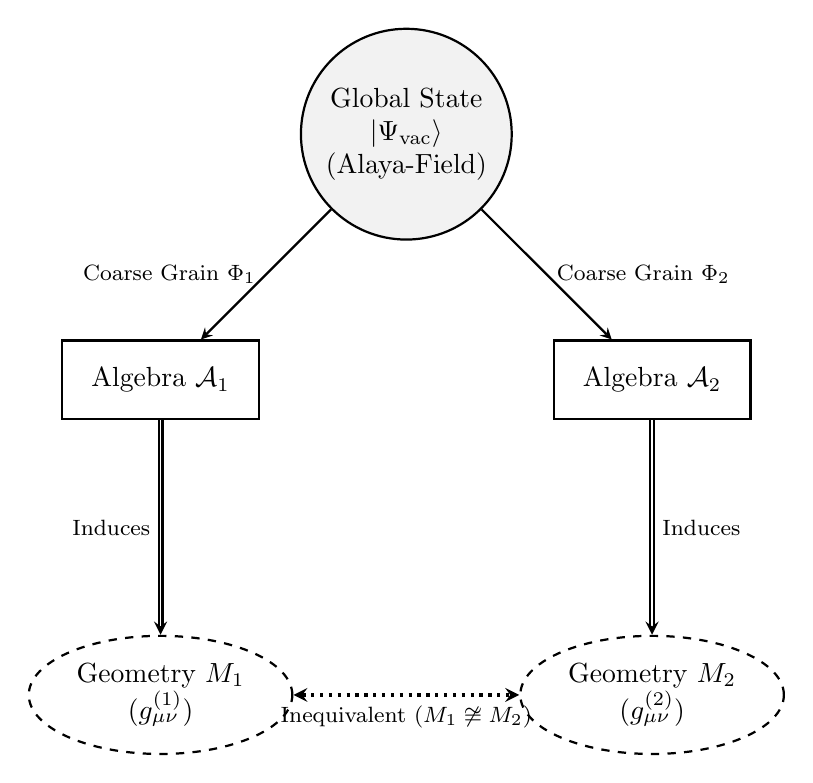
\begin{tikzpicture}[>=stealth, auto, node distance=3cm]
    % Styles
    \tikzstyle{state} = [circle, draw, thick, fill=gray!10, minimum size=2.5cm, align=center]
    \tikzstyle{filter} = [rectangle, draw, thick, fill=white, minimum width=2.5cm, minimum height=1cm]
    \tikzstyle{geo} = [ellipse, draw, thick, dashed, minimum width=2.5cm, minimum height=1.5cm, align=center]
    
    % Nodes
    \node[state] (Alaya) {Global State\\$|\Psi_{\text{vac}}\rangle$\\(Alaya-Field)};
    
    \node[filter] (Filter1) [below left of=Alaya, xshift=-1cm, yshift=-1cm] {Algebra $\mathcal{A}_1$};
    \node[filter] (Filter2) [below right of=Alaya, xshift=1cm, yshift=-1cm] {Algebra $\mathcal{A}_2$};
    
    \node[geo] (Geo1) [below of=Filter1, yshift=-1cm] {Geometry $M_1$\\($g_{\mu\nu}^{(1)}$)};
    \node[geo] (Geo2) [below of=Filter2, yshift=-1cm] {Geometry $M_2$\\($g_{\mu\nu}^{(2)}$)};
    
    % Arrows
    \draw[->, thick] (Alaya) -- node[left, font=\footnotesize] {Coarse Grain $\Phi_1$} (Filter1);
    \draw[->, thick] (Alaya) -- node[right, font=\footnotesize] {Coarse Grain $\Phi_2$} (Filter2);
    
    \draw[->, double, thick] (Filter1) -- node[left, font=\footnotesize] {Induces} (Geo1);
    \draw[->, double, thick] (Filter2) -- node[right, font=\footnotesize] {Induces} (Geo2);
    
    % Interaction
    \draw[<->, dotted, very thick] (Geo1) -- node[below, font=\footnotesize] {Inequivalent ($M_1 \not\cong M_2$)} (Geo2);

\end{tikzpicture}
\caption{Schematic of the HAFF structure. A single global state $|\Psi_{\text{vac}}\rangle$ (Alaya) projects into topologically distinct emergent spacetimes ($M_1, M_2$) depending on the choice of observable algebra ($\mathcal{A}_1, \mathcal{A}_2$). This illustrates that geometry is observer-dependent in the fundamental sense.}
\label{fig:haff_scheme}
\end{figure}

\section{Discussion}
\label{sec:discussion}

\subsection{Relation to Existing Frameworks}

The framework developed in this work is not intended as a replacement for existing interpretational or algebraic approaches to quantum theory.
Rather, it is best understood as orthogonal to several well-established lines of thought, addressing a distinct structural question.
In this section, we briefly clarify its relation to three representative frameworks:

\subsubsection{Relation to QBism}

QBism emphasizes the role of agents and their personal probability assignments in quantum theory, interpreting the quantum state as an expression of subjective belief rather than an objective property of a system.
In contrast, the present framework assumes a single, objective global quantum state throughout.
No agent-dependent elements enter the formalism, and no interpretational commitments regarding belief, experience, or decision theory are required.

The point of contact lies solely in the rejection of a privileged subsystem decomposition.
While QBism attributes this absence to the primacy of the agent, our framework treats it as a structural feature of quantum theory itself.
Coarse-grainings are not chosen by agents, but instantiated by concrete physical interaction structures.
The resulting multiplicity of effective descriptions reflects physical underdetermination rather than subjectivity.

\subsubsection{Relation to Many-Worlds and Decoherence-Based Approaches}

Many-Worlds--type interpretations and decoherence-based accounts provide a compelling explanation of classical behavior within quantum mechanics by analyzing branching structures relative to a fixed subsystem decomposition.
Our framework does not modify this analysis, nor does it introduce an alternative account of branching or classicality.

The difference lies at a prior level.
Decoherence theory presupposes a tensor factorization into system, apparatus, and environment.
Here, we instead ask how such subsystem structures arise in the first place.
In this sense, the framework is complementary to decoherence-based approaches: it leaves their dynamical conclusions intact while removing subsystem factorization from the list of fundamental assumptions.

\subsubsection{Relation to Algebraic Quantum Field Theory}

The closest structural affinity of the present work is with algebraic quantum field theory (AQFT).
In AQFT, observable algebras are taken as primary, and states are defined as positive linear functionals over these algebras, without reliance on a global tensor product structure.
Our use of observable algebras and their representations is directly inspired by this tradition.

The present framework may be viewed as extending this algebraic perspective by emphasizing the role of coarse-graining relations between algebras.
Different choices of coarse-graining induce different effective representations and, consequently, different entanglement structures.
The novelty lies not in the algebraic formalism itself, but in using it to analyze the emergence and non-uniqueness of geometric descriptions.

Taken together, these comparisons situate the present work as a structural investigation into the conditions under which subsystem structure and geometry emerge.
It neither commits to a particular interpretation of quantum mechanics nor proposes a new dynamical law, but instead clarifies how several existing frameworks implicitly rely on assumptions that can be made explicit and, in some cases, relaxed.

\subsection{Scope and Limitations}

The present work is concerned with structural consistency rather than phenomenological prediction. 
Observable consequences depend on the physical mechanisms implementing a given coarse-graining, which lie beyond the scope of this paper. 
This is analogous to effective field theory, where multiple UV completions may share the same low-energy structure. 
Future work will explore concrete physical realizations and their empirical signatures.

\subsection{Philosophical Implications}

We emphasize that the framework assumes a single, objective global quantum state $|\Psi_U\rangle$. 
What is coarse-graining--dependent is not reality itself, but the effective structures used to describe it. 
This position is compatible with scientific realism while acknowledging the role of operational context in physical description.

\subsection{Future Directions}

While the present work is deliberately limited to a structural analysis of subsystem emergence and geometry within a fixed global quantum state, it naturally opens several directions for further investigation. 
We emphasize that the following points are not results established here, but rather indicate possible extensions where the current framework may provide useful conceptual or technical guidance.

\subsubsection{Dynamical Models of Coarse-Graining Selection}

In this work, coarse-graining structures are treated as fixed relational inputs, instantiated by concrete physical interaction patterns. 
A natural next step is to investigate whether such coarse-grainings can themselves be characterized dynamically.

One possible direction is to study how interaction Hamiltonians, coupling strengths, or network topologies bias the emergence of particular subalgebra structures over others. 
This could clarify under what physical conditions certain factorizations become robust or persistent, and whether transitions between inequivalent coarse-grainings admit an effective dynamical description.

Importantly, such an analysis would remain compatible with globally unitary evolution, treating coarse-graining selection as an emergent, effective phenomenon rather than a modification of fundamental dynamics.

\subsubsection{Connections to Quantum Information and Complexity}

The non-uniqueness of emergent geometry highlighted here suggests a close connection to quantum information--theoretic notions such as entanglement structure, operator complexity, and resource constraints.

Future work could explore whether preferred geometric descriptions correlate with informational criteria---for example, minimal description length, stability under noise, or computational accessibility of observables. 
Such considerations may help explain why certain coarse-grainings are physically salient, even when many are formally admissible.

This perspective may also provide a bridge to recent work on complexity-based approaches to spacetime emergence, without committing to any particular complexity measure at the present stage.

\subsubsection{Extensions to Quantum Field Theory and Continuum Limits}

While the framework has been formulated in abstract Hilbert space terms, an important open question concerns its implementation in quantum field--theoretic settings, where issues of locality, algebraic nets, and continuum limits arise.

In particular, it would be valuable to examine how coarse-graining relations between observable algebras interact with the locality structures emphasized in algebraic quantum field theory, and whether familiar spacetime geometries can be recovered as stable fixed points of such relations.

We stress that the present work does not resolve these questions, but provides a structural language in which they can be posed more precisely.

\subsubsection{Empirical and Phenomenological Implications}

At the level developed here, the framework is primarily structural and conceptual. 
Nevertheless, future investigations may ask whether different coarse-graining choices lead to distinguishable effective descriptions, for example in semiclassical regimes, quantum gravity--motivated models, or analogue systems.

Such studies could clarify whether the non-uniqueness of emergent geometry has observable consequences, or whether physical constraints effectively suppress this freedom in realistic settings.

Any empirical analysis would necessarily require additional assumptions beyond those adopted in this work, and thus lies outside its present scope.

\subsubsection{Conceptual Clarifications and Interpretational Interfaces}

Finally, although the framework is intentionally neutral with respect to interpretations of quantum mechanics, it may serve as a useful interface for comparative studies. 
By making explicit the structural assumptions underlying subsystem decomposition and geometry, it could help clarify which features are interpretation-dependent and which arise more generally from the formalism itself.

We view this not as an attempt to adjudicate between interpretations, but as an opportunity to sharpen the questions they address.

\medskip

Taken together, these directions suggest that the framework developed here is best viewed as a scaffold: it does not dictate specific physical models, but provides a structured setting in which questions about subsystems, geometry, and emergence can be formulated with greater precision.

\section{Conclusion}
\label{sec:conclusion}

We have presented a framework in which subsystem structure is not presupposed, but emerges from coarse-graining over observable algebras. 
The central results are:

\begin{enumerate}
\item A generic quantum state admits no canonical tensor factorization (Theorem~\ref{thm:nofact}).
\item Different coarse-graining structures induce inequivalent effective subsystem descriptions (Theorem~\ref{thm:inequiv}).
\item These inequivalent coarse-grainings generically give rise to distinct emergent geometries (Theorem~\ref{thm:geom}), and this distinction cannot be reduced to coordinate choice.
\end{enumerate}

The framework is deliberately limited in scope. 
We have not proposed new dynamics, derived empirical predictions, or resolved interpretational debates. 
Instead, we have examined the structural consequences of removing subsystem factorization from the list of fundamental assumptions.

This investigation reveals that the emergence of geometry is more context-dependent than often acknowledged. 
Geometry is not an intrinsic property of a quantum state alone, but depends on how information is rendered accessible through coarse-graining. 
This perspective is compatible with, and complementary to, existing approaches including decoherence theory, holographic duality, and algebraic quantum field theory.

Several open questions remain. 
Can coarse-graining structures themselves be characterized dynamically? 
Do informational or complexity-based criteria select physically preferred coarse-grainings? 
Can the framework be extended to quantum field theory and reconciled with standard locality structures? 
These questions lie beyond the present scope, but the structural setting developed here provides a language in which they can be formulated with greater precision.

Ultimately, this work suggests that the relationship between quantum states, subsystems, and geometry is more subtle than the standard picture implies. 
By making explicit an assumption that is often left implicit, we hope to have clarified the conditions under which emergence occurs and opened new avenues for investigating the foundations of quantum theory and spacetime.

\section*{Acknowledgments}

The author thanks the anonymous reviewers for their insightful comments and suggestions, which greatly improved the clarity and rigor of this work.

\begin{thebibliography}{99}

\bibitem{Zurek2003}
W. H. Zurek, \emph{Decoherence, einselection, and the quantum origins of the classical}, Rev. Mod. Phys. \textbf{75}, 715 (2003).

\bibitem{Maldacena1999}
J. M. Maldacena, \emph{The Large N limit of superconformal field theories and supergravity}, Int. J. Theor. Phys. \textbf{38}, 1113 (1999).

\bibitem{VanRaamsdonk2010}
M. Van Raamsdonk, \emph{Building up spacetime with quantum entanglement}, Gen. Relativ. Gravit. \textbf{42}, 2323 (2010).

\bibitem{RyuTakayanagi2006}
S. Ryu and T. Takayanagi, \emph{Holographic Derivation of Entanglement Entropy from AdS/CFT}, Phys. Rev. Lett. \textbf{96}, 181602 (2006).

\bibitem{Zanardi2001}
P. Zanardi, \emph{Virtual Quantum Subsystems}, Phys. Rev. Lett. \textbf{87}, 077901 (2001).

\bibitem{Zanardi2004}
P. Zanardi, D. A. Lidar, and S. Lloyd, \emph{Quantum Tensor Product Structures are Observable Induced}, Phys. Rev. Lett. \textbf{92}, 060402 (2004).

\bibitem{Viola2004}
H. Barnum, E. Knill, G. Ortiz, R. Somma, and L. Viola, \emph{A Subsystem-Independent Generalization of Entanglement}, Phys. Rev. Lett. \textbf{92}, 107902 (2004).

\bibitem{Haag1996}
R. Haag, \emph{Local Quantum Physics: Fields, Particles, Algebras}, Springer-Verlag (1996).

\bibitem{Page1993}
D. N. Page, \emph{Average entropy of a subsystem}, Phys. Rev. Lett. \textbf{71}, 1291 (1993).

\bibitem{Petz1996}
D. Petz, \emph{Monotone metrics on matrix spaces}, Linear Algebra Appl. \textbf{244}, 81 (1996).

\bibitem{Swingle2012}
B. Swingle, \emph{Entanglement Renormalization and Holography}, Phys. Rev. D \textbf{86}, 065007 (2012).

\end{thebibliography}

\end{document}